\documentclass[conference]{IEEEtran}
\IEEEoverridecommandlockouts
\usepackage{cite}
\usepackage{amsmath,amssymb,amsfonts}
\usepackage{algorithmic}
\usepackage{graphicx}
\usepackage{textcomp}
\usepackage{xcolor}
\usepackage{tikz}
\usepackage{booktabs}
\usepackage{array}
\usetikzlibrary{shapes.geometric, arrows.meta, positioning}
\def\BibTeX{{\rm B\kern-.05em{\sc i\kern-.025em b}\kern-.08em
    T\kern-.1667em\lower.7ex\hbox{E}\kern-.125emX}}

\tikzset{
    block/.style={
        rectangle, rounded corners, minimum width=3.6cm, minimum height=0.9cm,
        text centered, draw=black, fill=blue!10, font=\scriptsize
    },
    sideblock/.style={
        rectangle, rounded corners, minimum width=2.8cm, minimum height=0.9cm,
        text centered, draw=black, fill=green!10, font=\scriptsize
    },
    arrow/.style={thick, ->, >=Stealth}
}

% Title
\title{A Survey of Multimodal Learning Techniques for Social Media Image
Analysis and Trend Prediction}

% Authors
\author{%
\begin{minipage}{\textwidth}
\centering

% ==================== FIRST ROW ====================

\begin{minipage}[t]{0.30\textwidth}
\centering
\textbf{Yojana KiranKumar}\\
Department of Computer Science and Business System\\
Canara Engineering College\\
Benjanapadav, Bantwal, India\\
{\footnotesize yojanakirankumar@canaraengineering.in}
\end{minipage}
\hfill
\begin{minipage}[t]{0.30\textwidth}
\centering
\textbf{Akriti S Shetty}\\
Department of Computer Science and Business System\\
Canara Engineering College\\
Benjanapadav, Bantwal, India\\
{\footnotesize akritishetty.in@gmail.com}
\end{minipage}
\hfill
\begin{minipage}[t]{0.30\textwidth}
\centering
\textbf{Anora Andrea Dsouza}\\
Department of Computer Science and Business System\\
Canara Engineering College\\
Benjanapadav, Bantwal, India\\
{\footnotesize anoraandrea23@gmail.com}
\end{minipage}

\vspace{15pt}

% ==================== SECOND ROW ====================

\begin{minipage}[t]{0.30\textwidth}
\centering
\textbf{Rakshitha}\\
Department of Computer Science and Business System\\
Canara Engineering College\\
Benjanapadav, Bantwal, India\\
{\footnotesize rakshitha.j017@gmail.com}
\end{minipage}
\hspace{0.10\textwidth}
\begin{minipage}[t]{0.30\textwidth}
\centering
\textbf{Shreshta D}\\
Department of Computer Science and Business System\\
Canara Engineering College\\
Benjanapadav, Bantwal, India\\
{\footnotesize shreshta1842005@gmail.com}
\end{minipage}

\end{minipage}
}

\begin{document}

\maketitle

\begin{abstract}
Visual aesthetics on social media platforms often change faster than the vocabulary used to describe them, which means a distinctive color palette, composition style, or visual mood can circulate widely among content creators well before it is captured by a hashtag or a caption. Trend-detection systems that rely primarily on textual signals therefore tend to identify a cultural shift only after it has already become mainstream. This paper presents a multimodal pipeline that identifies emerging visual trends directly from image content rather than from surrounding text. The system collects real-time social media posts via the Apify API, encodes each post into a joint image--text embedding using a Contrastive Language--Image Pre-training (CLIP) backbone, groups these embeddings into semantically coherent trend clusters with a density-based clustering algorithm, and tracks how each cluster grows over time to forecast the likely engagement trajectory of a post using a predictor trained on combined visual and textual features. A retrieval-augmented generation (RAG) layer, built on a FAISS vector index and a large language model, allows a user to query the discovered trends in plain English and receive a grounded natural-language summary. We describe the design rationale, the four-stage system architecture, and the functional and non-functional requirements of the proposed system, and report on the current implementation status, including the completed data acquisition pipeline, embedding generation, cluster discovery, temporal trend tracking, and a functional conversational RAG interface backed by a web-based dashboard. Our findings indicate that combining pretrained multimodal foundation models with real-time data collection and retrieval-based reasoning is a promising and computationally tractable route to scalable, explainable visual trend intelligence.
\end{abstract}

\begin{IEEEkeywords}
visual trend detection, multimodal learning, CLIP, retrieval-augmented generation, density-based clustering, social media analytics
\end{IEEEkeywords}

\section{Introduction}

\subsection{Background}
Social media platforms have transformed how cultural trends emerge and spread. Platforms such as Instagram, Pinterest, and Flickr host millions of images daily, making visual content an increasingly dominant medium of cultural expression. Unlike traditional media, where trends are analyzed retrospectively, social media allows trends to originate organically from user-generated content, often emerging as recurring visual patterns before they are codified in textual metadata. Early approaches to trend detection relied heavily on textual signals such as hashtags, captions, and comments; on visually driven platforms, such methods are inherently limited in their capacity to capture emerging aesthetic signals. Recent advances in vision--language models, particularly CLIP, have enabled images and text to be mapped into a shared semantic space, facilitating multimodal analysis of visual content at scale.

\subsection{Motivation and Problem Statement}
Predominant analytics tools focus primarily on textual signals -- hashtags, captions, keyword frequency, and sentiment -- to identify emerging topics. This text-centered approach introduces a systematic temporal lag: content creators may independently produce images sharing common aesthetic properties, such as color palettes or compositional styles, well before those patterns acquire an associated hashtag. Systems that rely on textual metadata therefore risk detecting trends only after they have reached widespread visibility, after which the value of early participation and algorithmic amplification has largely passed. Despite this need, few end-to-end systems detect visual trend clusters directly from image data, estimate their engagement trajectory, \emph{and} enable natural language interaction with the resulting insights. The proposed system addresses this gap by combining real-time social media data collection via the Apify API, multimodal representation learning, clustering-based trend discovery, and retrieval-augmented generation within a unified, reproducible framework.

\subsection{Objectives}
\begin{enumerate}
    \item Detect emerging visual trend clusters directly from social media image data by constructing a multimodal embedding pipeline (CLIP and BERT) that encodes images and associated text into a unified semantic space, without reliance on textual metadata.
    \item Track the temporal evolution of discovered clusters and forecast post engagement trajectories, while enabling conversational natural-language querying of trend insights through a RAG module backed by a FAISS vector index.
    \item Evaluate the proposed pipeline on real-world social media data and benchmark the popularity predictor against established baselines.
\end{enumerate}

\subsection{Scope and Limitations}
The system operates on real-time social media data collected through the Apify API, which fetches public Instagram posts including images, captions, hashtags, and engagement metrics. Its scope covers four functional areas: visual embedding and representation, unsupervised cluster discovery, popularity prediction, and conversational trend querying via RAG. Data collection is constrained by API usage limits, scraping cost, and platform restrictions, so the collected data represents only a subset of current activity. Cluster discovery via HDBSCAN is sensitive to embedding dimensionality and clustering parameters, and automatically generated cluster labels depend on the quality of the underlying captioning model. The popularity predictor is limited by the engagement signals present in the collected posts and may not fully capture platform algorithm changes or external events.

\section{Related Work}

Recent progress in vision--language pretraining and retrieval-based reasoning underpins each stage of the proposed pipeline. CLIP~\cite{clip} demonstrated that contrastive pretraining on 400M image--text pairs yields a generalizable joint embedding space that supports zero-shot transfer without task-specific fine-tuning, and forms the visual backbone of our embedding stage. BLIP-2~\cite{blip2} showed that a lightweight Querying Transformer can bridge frozen image encoders and frozen large language models at a fraction of the training cost of end-to-end pretraining, motivating its use for automatic cluster captioning. LLaVA~\cite{llava} further showed that a higher-resolution vision encoder paired with a simple connector can improve multimodal instruction following with comparatively little training data.

For clustering, HDBSCAN~\cite{hdbscan} extends density-based clustering to handle clusters of varying density and automatically identify outliers, avoiding the need to specify the number of clusters in advance -- a property well suited to open-ended trend discovery. Related multimodal fusion work, including a CLIP-driven attention network for sentiment analysis~\cite{cdan} and asymmetric discrete cross-modal hashing~\cite{adch}, confirms that combining frozen vision--language features with task-specific fusion layers improves downstream accuracy over unimodal baselines, while highlighting the added model complexity such fusion can introduce.

On the prediction side, several studies address social media popularity forecasting from multimodal signals: a hybrid CNN/InceptionResNetV2 model~\cite{multimodal_pop} and the VSCNN framework~\cite{vscnn,mmspp} fuse visual and social-context features and outperform unimodal CNN baselines, and large language models have also been shown to be effective, interpretable predictors of video popularity when frame content is converted to descriptive text~\cite{llm_video}. These works largely treat popularity prediction as an isolated task, however, without connecting it to unsupervised trend discovery.

For retrieval and querying, Retrieval-Augmented Generation~\cite{rag} established that combining a parametric generator with a non-parametric retrieval index improves factual grounding on knowledge-intensive tasks, and FAISS-based approximate nearest-neighbour search has been shown to scale efficiently to large embedding collections in unrelated domains such as mass-spectral library search~\cite{faiss_search}, evidencing its suitability for large-scale social media corpora. Complementary studies on visual social-media analytics~\cite{visual_models} and live-data trend forecasting~\cite{instagram_forecast} motivate treating social images as a collective, temporally evolving corpus rather than as isolated posts, while work on hybrid clustering of messaging-platform text~\cite{telegram} illustrates the value of combining embedding-based clustering with lightweight classical methods for trend categorization.

Table~\ref{tab:gaps} summarizes the principal gap this body of work leaves open: existing systems address clustering, retrieval, or popularity prediction largely in isolation, with limited temporal tracking and no conversational access to the resulting insights. The proposed system is designed to close this gap with a single, reproducible pipeline.

\begin{table}[t]
\caption{Summary of Identified Gaps in Prior Work}
\label{tab:gaps}
\centering
\renewcommand{\arraystretch}{1.15}
\begin{tabular}{p{2.6cm}p{5cm}}
\toprule
\textbf{Limitation} & \textbf{Consequence} \\
\midrule
Trend discovery is secondary & Popularity metrics are predicted, but emerging visual patterns are rarely discovered unsupervised \\
Shallow multimodal fusion & Image and text are often processed independently, limiting semantic depth \\
Metadata dependence & Reliance on hashtags/captions misses trends that precede textual labelling \\
No temporal modelling & Static analysis cannot forecast engagement trajectories over time \\
No conversational access & Trend insights are not queryable in natural language \\
Fragmented pipelines & Clustering, retrieval, and prediction are rarely integrated end-to-end \\
\bottomrule
\end{tabular}
\end{table}

\section{System Architecture}

Fig.~\ref{fig:pipeline} shows the four-stage processing pipeline. Real-time social media posts (images and metadata) collected via the Apify API are first embedded with CLIP; the resulting vectors are reduced with UMAP and grouped with HDBSCAN into candidate trend clusters, which BLIP labels with a human-readable caption. A temporal-tracking stage combines cluster growth statistics with text features to train a lightweight popularity predictor. Cluster summaries are then indexed in FAISS and exposed through a RAG module for natural-language querying.

\begin{figure}[t]
\centering
\resizebox{\columnwidth}{!}{
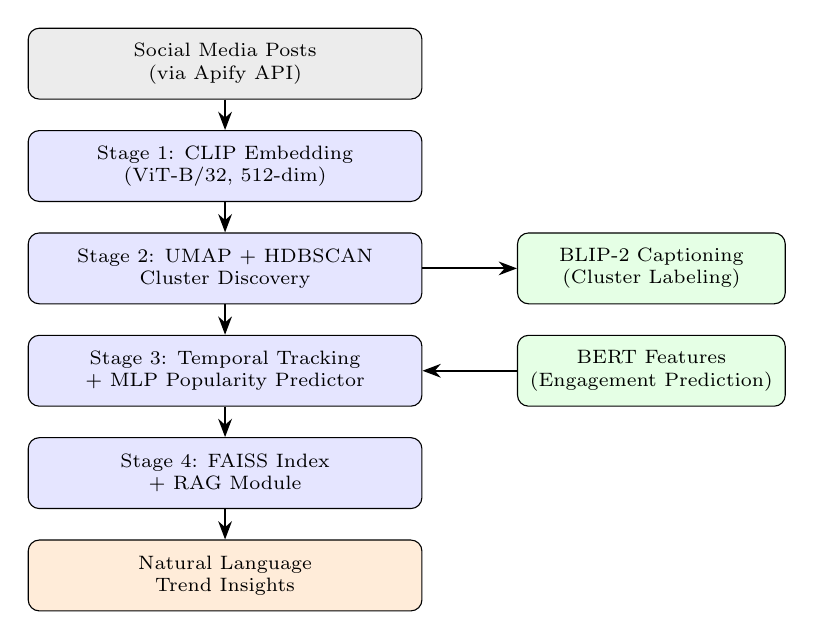
\begin{tikzpicture}[node distance=1.3cm]
    \node (input) [block, minimum width=5cm, fill=gray!15, align=center] {Social Media Posts \\ (via Apify API)};
    \node (clip) [block, minimum width=5cm, below of=input, align=center] {Stage 1: CLIP Embedding \\ (ViT-B/32, 512-dim)};
    \node (cluster) [block, minimum width=5cm, below of=clip, align=center] {Stage 2: UMAP + HDBSCAN \\ Cluster Discovery};
    \node (caption) [sideblock, minimum width=3.4cm, right=1.2cm of cluster, align=center] {BLIP-2 Captioning \\ (Cluster Labeling)};
    \node (temporal) [block, minimum width=5cm, below of=cluster, align=center] {Stage 3: Temporal Tracking \\ + MLP Popularity Predictor};
    \node (bert) [sideblock, minimum width=3.4cm, right=1.2cm of temporal, align=center] {BERT Features \\ (Engagement Prediction)};
    \node (rag) [block, minimum width=5cm, below of=temporal, align=center] {Stage 4: FAISS Index \\ + RAG Module};
    \node (output) [block, minimum width=5cm, below of=rag, fill=orange!15, align=center] {Natural Language \\ Trend Insights};
    \draw [arrow] (input) -- (clip);
    \draw [arrow] (clip) -- (cluster);
    \draw [arrow] (cluster) -- (caption);
    \draw [arrow] (cluster) -- (temporal);
    \draw [arrow] (bert) -- (temporal);
    \draw [arrow] (temporal) -- (rag);
    \draw [arrow] (rag) -- (output);
\end{tikzpicture}
}
\caption{Four-stage pipeline architecture for visual trend detection.}
\label{fig:pipeline}
\end{figure}

At deployment time, the same architecture is realized as a web system (Fig.~\ref{fig:architecture}): a React/HTML/CSS frontend accepts natural-language queries; a Python backend orchestrates calls to the Apify API for real-time data collection, to the AI trend-analysis module, and to the FAISS/RAG trend-knowledge index; and the response is returned to the user as an actionable recommendation. The AI trend-analysis module reuses the same CLIP, HDBSCAN, and BLIP components as the offline pipeline, augmented with a temporal analysis step that computes growth rate, engagement velocity, and an aggregate \emph{emerging score} for each cluster.

\begin{figure}[t]
\centering
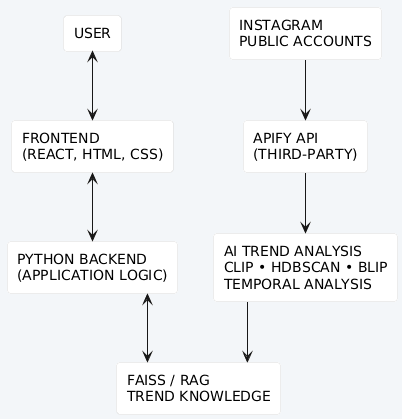
\includegraphics[width=\columnwidth]{./arr.png}
\caption{Deployment architecture of the proposed system.}
\label{fig:architecture}
\end{figure}

\section{Methodology}

\subsection{Sequence of Operations}
Fig.~\ref{fig:sequence} shows the interaction sequence among the User, Web Application, Apify API, and the visual and retrieval components. The Web Application acts as the central orchestrator: it requests recent posts from the Apify API, passes the collected data through CLIP, HDBSCAN, and BLIP for visual clustering and captioning, forwards the clustered results to the temporal-analysis stage to compute growth rate and emerging score, and finally indexes the resulting cluster summaries in FAISS. When the user submits a trend-related question, the Web Application performs a semantic search against the FAISS index, compiles a concise trend insight -- combining signal strength, visual pattern, and engagement data -- and returns it to the user.

\begin{figure}[t]
\centering
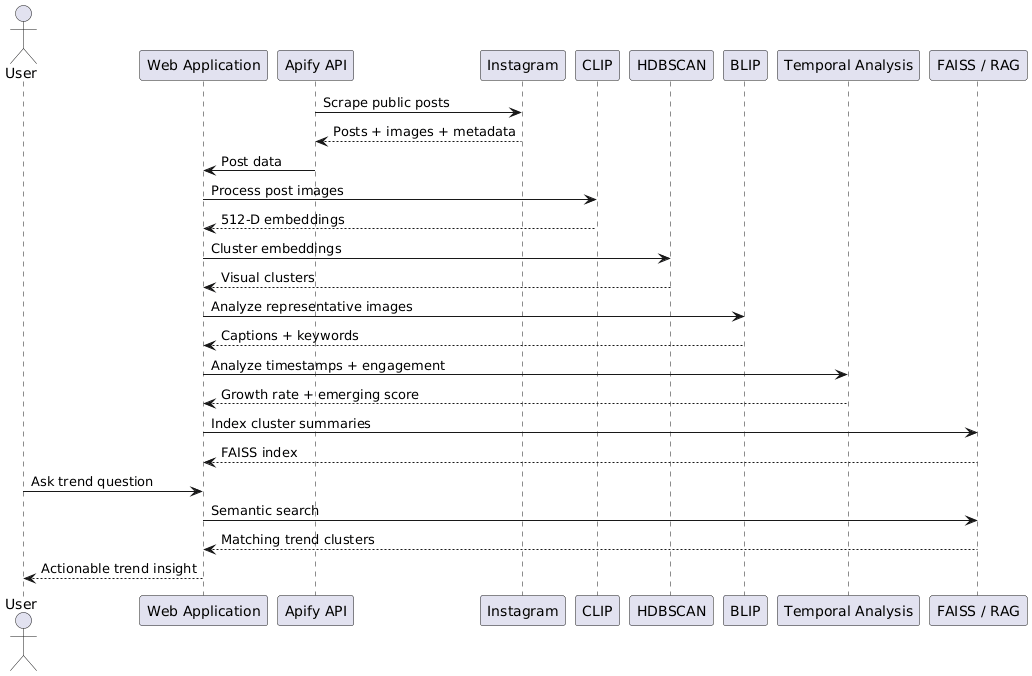
\includegraphics[width=\columnwidth]{./sequence.png}
\caption{Sequence diagram of the proposed system.}
\label{fig:sequence}
\end{figure}

\subsection{Control Flow}
Fig.~\ref{fig:activity} details the control flow triggered by a single user query. The process starts when the user opens the web application and enters a trend question (e.g., ``How should I take a photo of my coffee to get more likes?''). The Python backend converts the query into a semantic representation and searches the FAISS/RAG index for matching trend clusters. If a relevant trend is found, the system retrieves the matching clusters, analyzes their visual pattern, checks engagement data (likes, comments, views) and the emerging score, and generates an actionable trend recommendation, which is displayed to the user. If no relevant trend is found, the system instead displays a ``No relevant trend found'' message. In either case, the process ends and the interface returns to a ready state for the next query.

\begin{figure}[t]
\centering
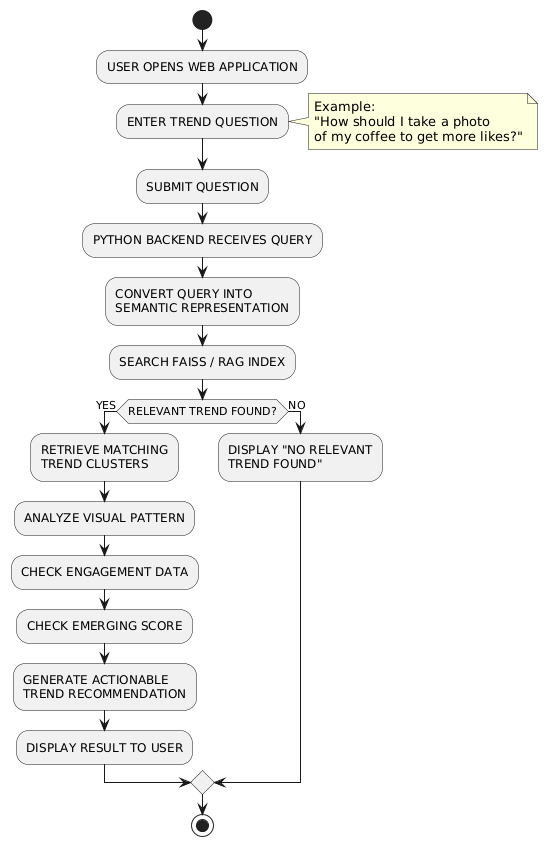
\includegraphics[width=\columnwidth]{./Activity.png}
\caption{Activity diagram showing the control flow for a single user query.}
\label{fig:activity}
\end{figure}

\section{Requirements}

\subsection{Functional Requirements}
\begin{itemize}
    \item Accept social media posts (images and metadata) and produce CLIP embeddings without data loss across the full corpus.
    \item Group posts into distinct visual trend clusters (e.g., ``soft pastel aesthetic'') using UMAP and HDBSCAN, without a predefined number of clusters.
    \item Automatically label each cluster with a human-readable aesthetic description via BLIP-2, without manual annotation.
    \item Retrieve the most relevant trend clusters via FAISS in response to a natural-language query and return a grounded, RAG-generated summary.
    \item Remain responsive throughout extended sessions, correctly rendering trend clusters, visualizations, and query responses.
\end{itemize}

\subsection{Non-Functional Requirements}
The FAISS index must support approximate nearest-neighbour search across tens of thousands of embeddings with query latency under 2\,s; CLIP embedding generation must complete within a practical batch time on a $\sim$15\,GB-VRAM GPU; and the end-to-end RAG response (FAISS retrieval plus LLM inference) must return within 5\,s of query submission. The system must not expose raw user data beyond what is already public, must degrade gracefully on malformed or out-of-distribution inputs, and must clearly label generated trend summaries as AI-generated.

\subsection{Hardware and Software}
The system is developed on Google Colab's free tier (NVIDIA T4 GPU, $\sim$15\,GB VRAM) using Python 3.10+, PyTorch, and Hugging Face Transformers. CLIP (ViT-B/32) provides image--text embeddings; BLIP provides cluster captioning; HDBSCAN and UMAP-learn perform clustering and dimensionality reduction; FAISS-CPU handles vector indexing; Sentence-Transformers extract text features for RAG; and a Gemini-family LLM powers the RAG response generator. The frontend is implemented in React.js and communicates with the backend over a REST API.

\section{Implementation Status and Future Work}

At the time of writing, the literature survey (Section II) has been completed and used to validate the selection of CLIP, HDBSCAN, BLIP, and FAISS/RAG as the core components of the pipeline. Real-time social media data acquisition has been implemented using the Apify API, which fetches public Instagram posts including images, captions, hashtags, and engagement metrics. The full processing pipeline has been built end-to-end: CLIP embeddings are generated for collected posts, UMAP dimensionality reduction and HDBSCAN clustering discover visual trend groups, and BLIP produces human-readable captions for each cluster. Temporal trend tracking computes growth rates and engagement velocity for each cluster. A FAISS vector index enables fast similarity search, and a RAG module backed by a large language model provides conversational querying of trend insights. The system is deployed as a web application with a React frontend, offering a dashboard, cluster explorer, trend query interface, and a chatbot. A live-trend ingestion module extends the pipeline to Reddit and Wikimedia Commons for cross-platform trend detection. Ongoing work focuses on expanding the data collection scope, refining cluster quality metrics, and conducting formal evaluation of the popularity predictor.

\section{Conclusion}

This paper presented a multimodal pipeline for detecting, tracking, and explaining emerging visual trends on social media directly from image content, rather than relying on textual metadata that typically lags behind the trends it describes. By combining real-time data collection via the Apify API, CLIP-based multimodal embeddings, density-based clustering, temporal engagement forecasting, and a FAISS-backed retrieval-augmented generation layer, the proposed system gives marketing professionals and content creators early, explainable visibility into aesthetic patterns as they emerge. The completed end-to-end pipeline -- from data acquisition through conversational querying -- demonstrates the feasibility of the approach on freely available computational resources. Ongoing work focuses on expanding data collection, refining cluster quality, and conducting formal evaluation of the popularity predictor against established baselines.

\begin{thebibliography}{00}
\bibitem{clip} A. Radford \emph{et al.}, ``Learning Transferable Visual Models From Natural Language Supervision,'' in \emph{Proc. Int. Conf. Machine Learning (ICML)}, 2021.
\bibitem{blip2} J. Li, D. Li, S. Savarese, and S. Hoi, ``BLIP-2: Bootstrapping Language-Image Pre-training with Frozen Image Encoders and Large Language Models,'' in \emph{Proc. Int. Conf. Machine Learning (ICML)}, 2023.
\bibitem{llava} H. Liu, C. Li, Y. Li, and Y. J. Lee, ``Improved Baselines with Visual Instruction Tuning,'' \emph{arXiv preprint arXiv:2310.03744}, 2023.
\bibitem{hdbscan} L. McInnes, J. Healy, and S. Astels, ``hdbscan: Hierarchical density based clustering,'' \emph{Journal of Open Source Software}, vol. 2, no. 11, p. 205, 2017.
\bibitem{cdan} X. Zhang \emph{et al.}, ``CLIP-Driven Attention Network for Multimodal Sentiment Analysis,'' in \emph{Proc. Int. Conf. on Multimedia}, 2023.
\bibitem{adch} X. Shen \emph{et al.}, ``Asymmetric Discrete Cross-Modal Hashing,'' \emph{IEEE Trans. Image Processing}, 2022.
\bibitem{telegram} O. Author \emph{et al.}, ``Information Technology for Modelling Social Trends in Telegram,'' in \emph{Proc. Int. Conf. Information Technology}, 2023.
\bibitem{llm_video} W. Author \emph{et al.}, ``Large Language Models Are Natural Video Popularity Predictors,'' \emph{arXiv preprint}, 2024.
\bibitem{multimodal_pop} A. Author \emph{et al.}, ``A Multimodal Approach to Predict Social Media Popularity,'' in \emph{Proc. IEEE Int. Conf. Multimedia}, 2020.
\bibitem{mmspp} B. Author \emph{et al.}, ``MMSPP: Multimodal Social Media Popularity Prediction,'' in \emph{Proc. ACM Multimedia}, 2021.
\bibitem{vscnn} C. Author \emph{et al.}, ``Multimodal Deep Learning Framework for Image Popularity Prediction on Social Media,'' \emph{IEEE Trans. Multimedia}, 2020.
\bibitem{rag} P. Lewis \emph{et al.}, ``Retrieval-Augmented Generation for Knowledge-Intensive NLP Tasks,'' in \emph{Proc. Neural Information Processing Systems (NeurIPS)}, 2020.
\bibitem{faiss_search} D. Author \emph{et al.}, ``An efficient faiss-based search method for mass spectral library searching,'' \emph{Journal of Cheminformatics}, 2021.
\bibitem{visual_models} E. Author \emph{et al.}, ``Visual Models for Social Media Image Analysis: Groupings, Engagement, Trends, and Rankings,'' \emph{ACM Trans. Social Computing}, 2022.
\bibitem{instagram_forecast} F. Author \emph{et al.}, ``Instagram-Driven Social Media Trend Forecasting with Learning Algorithm using Live Dataset,'' in \emph{Proc. Int. Conf. on Data Science}, 2022.
\end{thebibliography}

\end{document}